\section{Vehicel Kinematics and Dynamics}
\label{vehicle_kinematics_and_dynamics}

In this section, we will cover kinematic and dynamic modeling of an autonomous car. 
Creating a good vehicle model is essential for model-based control development. 
We'll look at modeling, both the evolution of the kinematics, that is, positions and velocities, and the dynamics or forces and torques of a car and how they connect. 
Later on in the next modules, we will use these vehicle models extensively for controller design. 


In this section, we will study

\begin{itemize}
\item Vehicle kinematics
\item Bicycle model
\item Longitudinal vehicle dynamics
\item Lateral vehicle dynamics
\end{itemize}

\begin{framed}
\theoremstyle{remark}
\begin{remark}{\textbf{Coordinate Transformations}}

Coordinate frames and transformations are explained in the appendix.
\end{remark}
\end{framed}

 
\subsection{Kinematic Modeling}
\label{kinematic_modeling}

So, let's get started. Generally, vehicle motion can be modeled either by considering the geometric constraint that defines its motion or by considering all of the forces and moments acting on a vehicle. 
The first case is known as Kinematic Modeling. Especially at low speeds when the accelerations are not significant, Kinematic Modeling is more than sufficient to capture the motion of a vehicle. When we instead include knowledge of the forces and moments acting on the vehicle, we're performing Dynamic Modeling. 
Dynamic models can do a great job of estimating vehicle motion throughout the vehicles operating range, but are more involved to develop than kinematic models. 

The robot's motion is constrained to move forward because its wheels point in this direction. 
This constraint is called a nonholonomic constraint, which means that it restricts the rate of change of the position of our robot. Mathematically, this can be expressed as follows:

\begin{equation}
\dot{y}\cos(\theta) - \dot{x}\sin(\theta) = 0
\end{equation} 


So, our robot can roll forward and turn while rolling, but cannot move sideways directly. We'll use this constraint to define a kinematic model for our robot. The velocity of the robot is defined by the tangent vector to its path see figure \ref{vehicle_path}. 

\begin{figure}[!htb]
\begin{center}
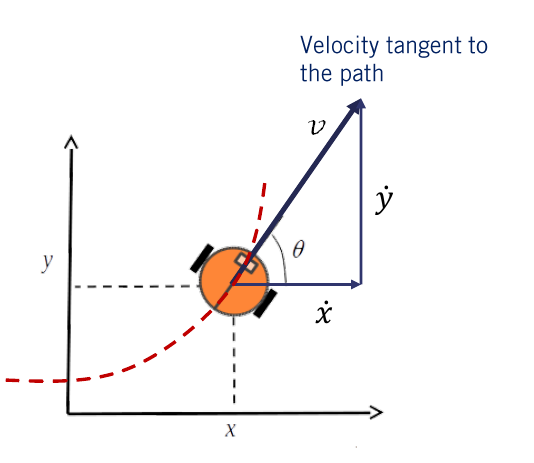
\includegraphics[scale=0.290]{img/kinematics/vehicle_path.jpeg}
\end{center}
\caption{Vehicle velocity.}
\label{vehicle_path}
\end{figure}


Let's define the orientation angle of the robot as $\theta$. Then $\tan(\theta)$ can be written as $dy$ over $dx$. 
The velocity of the robot in the y-direction divided by the velocity of the robot in the x-direction. 
By rearranging the above equation, we can derive an expression for the nonholonomic constraint equation as follows. 
We can then construct a pair of equations for the motion of the robot by combining these equations. 


\begin{equation}
\dot{x} = v \cos(\theta), ~~ \dot{y} = v\sin(\theta)
\end{equation}


We can assume the direct control over the robots rate of change of heading. We've now successfully built a kinematic model for our robot. This model takes as input the forward velocity in rotation rate and represents the robot using a vector of three states, the $x$ and $y$ position of the robot and it's heading. 


\begin{framed}
\theoremstyle{remark}
\begin{remark}{\textbf{State}}

A state is a set of variables often arranged in the form of a vector that fully describe the system at the current time.
\end{remark}
\end{framed}

The input of the model are velocity $v$ and rate of change of orientation $\omega$. 

\begin{figure}[!htb]
\begin{center}
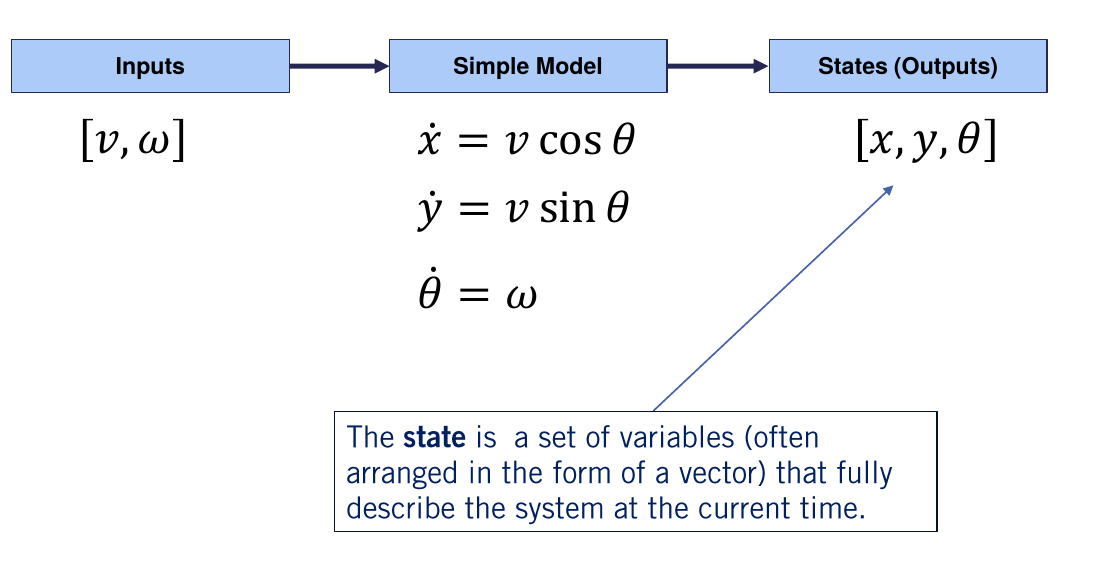
\includegraphics[scale=0.290]{img/kinematics/simple_robot_motion_kinematics.jpeg}
\end{center}
\caption{Simple robot motion kinematics.}
\label{simple_robot_motion_kinematics}
\end{figure}

However, for the actual two-wheel robot, it's also possible we need to directly command wheel velocities as inputs. We'll now look at how to extend our model and relate each wheel rotational velocity to forward velocity, $v$, and rotation rate $\omega$. We'll need a few more variables defined as follows. $P$ is the center of the robot, $L$ is the distance from the center of the robot to each of its wheels, $R$ is the radius of the wheels, $w_1$ and $w_2$ are the left and right wheel angular speeds. 

\begin{figure}[!htb]
\begin{center}
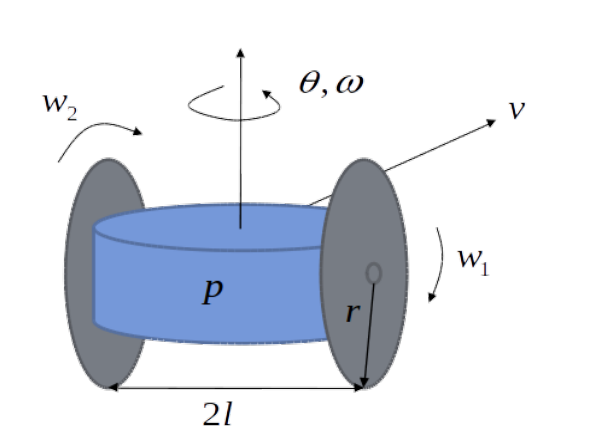
\includegraphics[scale=0.290]{img/kinematics/two_wheels_robot.jpeg}
\end{center}
\caption{Two wheels robot model.}
\label{two_wheels_robot}
\end{figure}


The velocity of the robot at each wheel is the radius of the wheel times its rotational velocity. 

\begin{equation}
 v =r \times w_i
\end{equation}

\begin{figure}[!htb]
\begin{center}
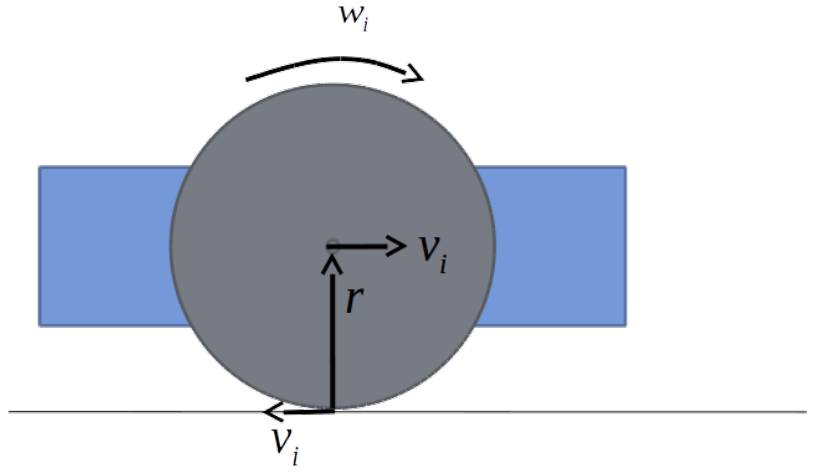
\includegraphics[scale=0.290]{img/kinematics/two_wheels_robot_kinematic_constraint.jpeg}
\end{center}
\caption{Two wheels robot model.}
\label{two_wheels_robot_kinematic_constraint}
\end{figure}

We can do this by assuming no slip between the wheel and the surface. The velocity of the robot can be computed as the average velocity of both wheels as seen from this figure. When the velocities of both wheels are the same, the robot moves in a straight line. If the wheel velocities are different, the robot moves in a curved path about some instantaneous center of rotation or ICR. We'll now use the notion of ICR to define the kinematic model for our two wheeled robot. We again have that the rotation rate $\omega$, is equal to $v$ over $r$, and can use similar triangles to define two expressions for Omega in terms of $v_2$ and Rho, and $v_1$, $v_2$ and $L$. Combining these equations with our expression for velocities $v_1$ and $v_2$ in terms of the wheel rotation speeds yields the final form of the equation for the rotation rate of the robot. We now return to our original robot model and substitute in the new expressions for the velocity and rotation rate of the two wheeled robot. We can see that the inputs of this model are $w_1$ and $w_2$, which are the wheel's angular speeds. The state remains the same for both robots. Also by discretizing the continuous time equations, we can convert our model from the differential form to a finite difference form. This form is convenient for controller design as we'll see shortly, as well as for simulation and state estimation purposes. Note that the subscript k means the value of the variables at the current time step, and the subscript k plus 1 will refer to values of the variables at the next time step. 


\begin{figure}[!htb]
\begin{center}
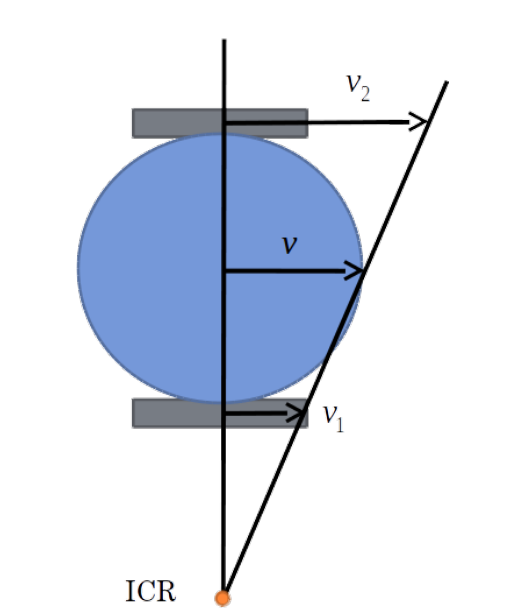
\includegraphics[scale=0.290]{img/kinematics/icr.jpeg}
\end{center}
\caption{Two wheels robot model.}
\label{icr}
\end{figure}

\begin{figure}[!htb]
\begin{center}
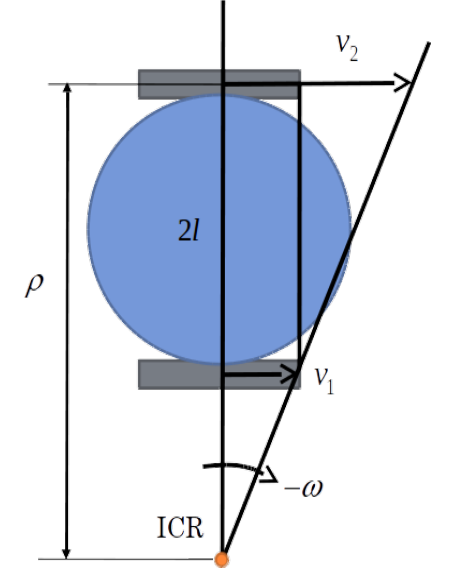
\includegraphics[scale=0.290]{img/kinematics/icr_II.jpeg}
\end{center}
\caption{Two wheels robot model.}
\label{icr_II}
\end{figure}




